\documentclass[11pt]{article}

\usepackage{graphicx}
\usepackage{url}

\begin{document}

\begin{titlepage}
	\begin{center}
    	
\includegraphics[scale=0.10]{du.png}\par
		\begin{Huge}
			\textsc{University of Dhaka}\par
		\end{Huge}
		\begin{Large}
			Department of Computer Science and Engineering\par \vspace{1cm}
			CSE-3111 : Computer Networking Lab \\[12pt]	
			Lab Report 1 :Lab exercises on LAN configuration and \\[5pt]  troubleshooting tools (PING, Traceroute, ARP, netstat, ifconfig, nslook,etc.)
		\end{Large}
	\end{center}  	
	\begin{large}
		\textbf{Submitted By:\\[12pt]}
			Name: Md Shamsur Rahman Sami\\[8pt]
			Roll No : 57\\[12pt]
			Name: Md Rakib Hossain\\[8pt]
			Roll No : 55\\[12pt]
		\textbf{Submitted On : \\[12pt]}
			January 26, 2024\\[20pt]
		\textbf{Submitted To :\\[12pt]}
			Dr. Md. Abdur Razzaque\\[12pt]
             
	\end{large}
\end{titlepage}

\section{Introduction}
In this comprehensive laboratory exercise focused on Local Area Network (LAN) configuration and troubleshooting tools. The lab delved into fundamental aspects of LAN setup, including ARP (Address Resolution Protocol), static routing, and configuration of network interfaces using tools such as Ifconfig. Troubleshooting skills were honed through the use of diagnostic utilities like PING and Traceroute, which enabled participants to identify and address connectivity issues. Additionally, participants gained insights into monitoring network activity with NETSTAT and resolving domain-related queries with NSLOOK. The lab fostered a practical understanding of essential networking tools, empowering participants with the knowledge and skills necessary for effective LAN configuration and troubleshooting.


%%%%
%%%%
\section{Theory}
In the realm of computer networking, Local Area Networks (LANs) play a pivotal role in connecting devices within a confined geographical area. The theory underlying LAN configuration revolves around the essential tasks of assigning IP addresses, configuring subnet masks, and establishing gateway addresses to facilitate seamless communication among networked devices. Address Resolution Protocol (ARP) becomes a critical component in this context, serving to map IP addresses to physical MAC addresses within the local network. Additionally, the concept of static routing involves the manual configuration of routing tables, offering a straightforward method for specifying network paths in environments where routing changes infrequently. The indispensable network utilities, PING and Traceroute, contribute to network troubleshooting and diagnostics by testing reachability and identifying the path to a destination, enhancing the overall understanding and management of LAN environments.



\section{Methodology}
\begin{itemize}
    \item  First open the cmd terminal in the windows system 
    \item  Run the following command in the terminal and get the output result and take the screenshot of the output.
    \begin{itemize}
    \item \textbf{IP Configuration:} \texttt{ipconfig}

    \item \textbf{PING:} \texttt{ping [IP address or hostname]}
    
    \item \textbf{Traceroute (Tracert in Windows):} \texttt{tracert [IP address or hostname]}
    
    \item \textbf{ARP (Address Resolution Protocol):} \texttt{arp -a}
    
    
    \item \textbf{Netstat (Network Statistics):} \texttt{netstat -a}
    
    \item \textbf{Nslookup (DNS Queries):} \texttt{nslookup [hostname or IP address]}
    
    % Add more commands in a similar format if needed
    
\end{itemize}

\end{itemize}


\section{Command Output}

Some Snapshots of the command output can be seen in the following figures: 

\subsection{}
\begin{figure}[!h]
\centering
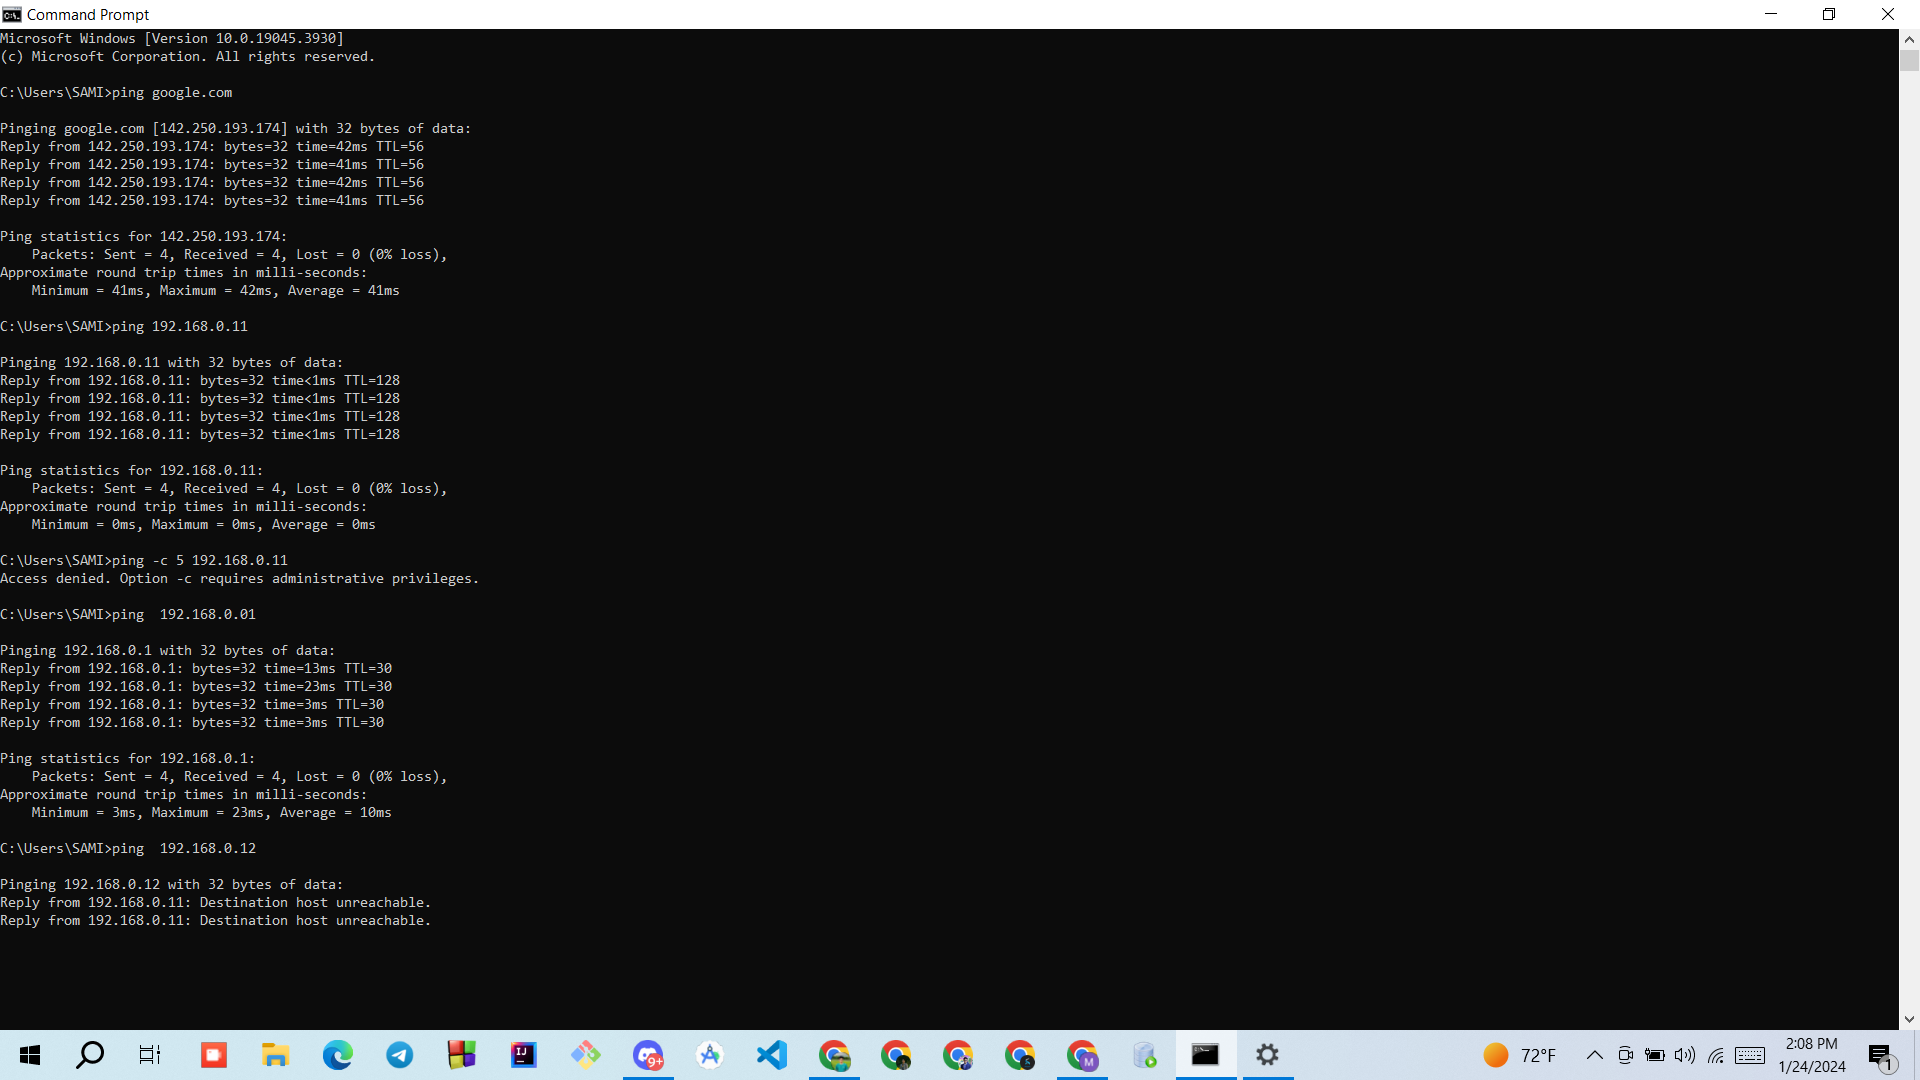
\includegraphics[width=\textwidth]{Screenshot (1).png}
\caption{PING Command}
\end{figure}

\begin{itemize}
  \item The `ping` command is a network utility used to check the availability and responsiveness of a host on an IP network.
  \item It sends ICMP Echo Request messages to the target, waits for Echo Replies, and displays round-trip time statistics.
  \item This tool is crucial for troubleshooting network connectivity and measuring latency.
\end{itemize}

\subsection{}
\begin{figure}[!h]
\centering
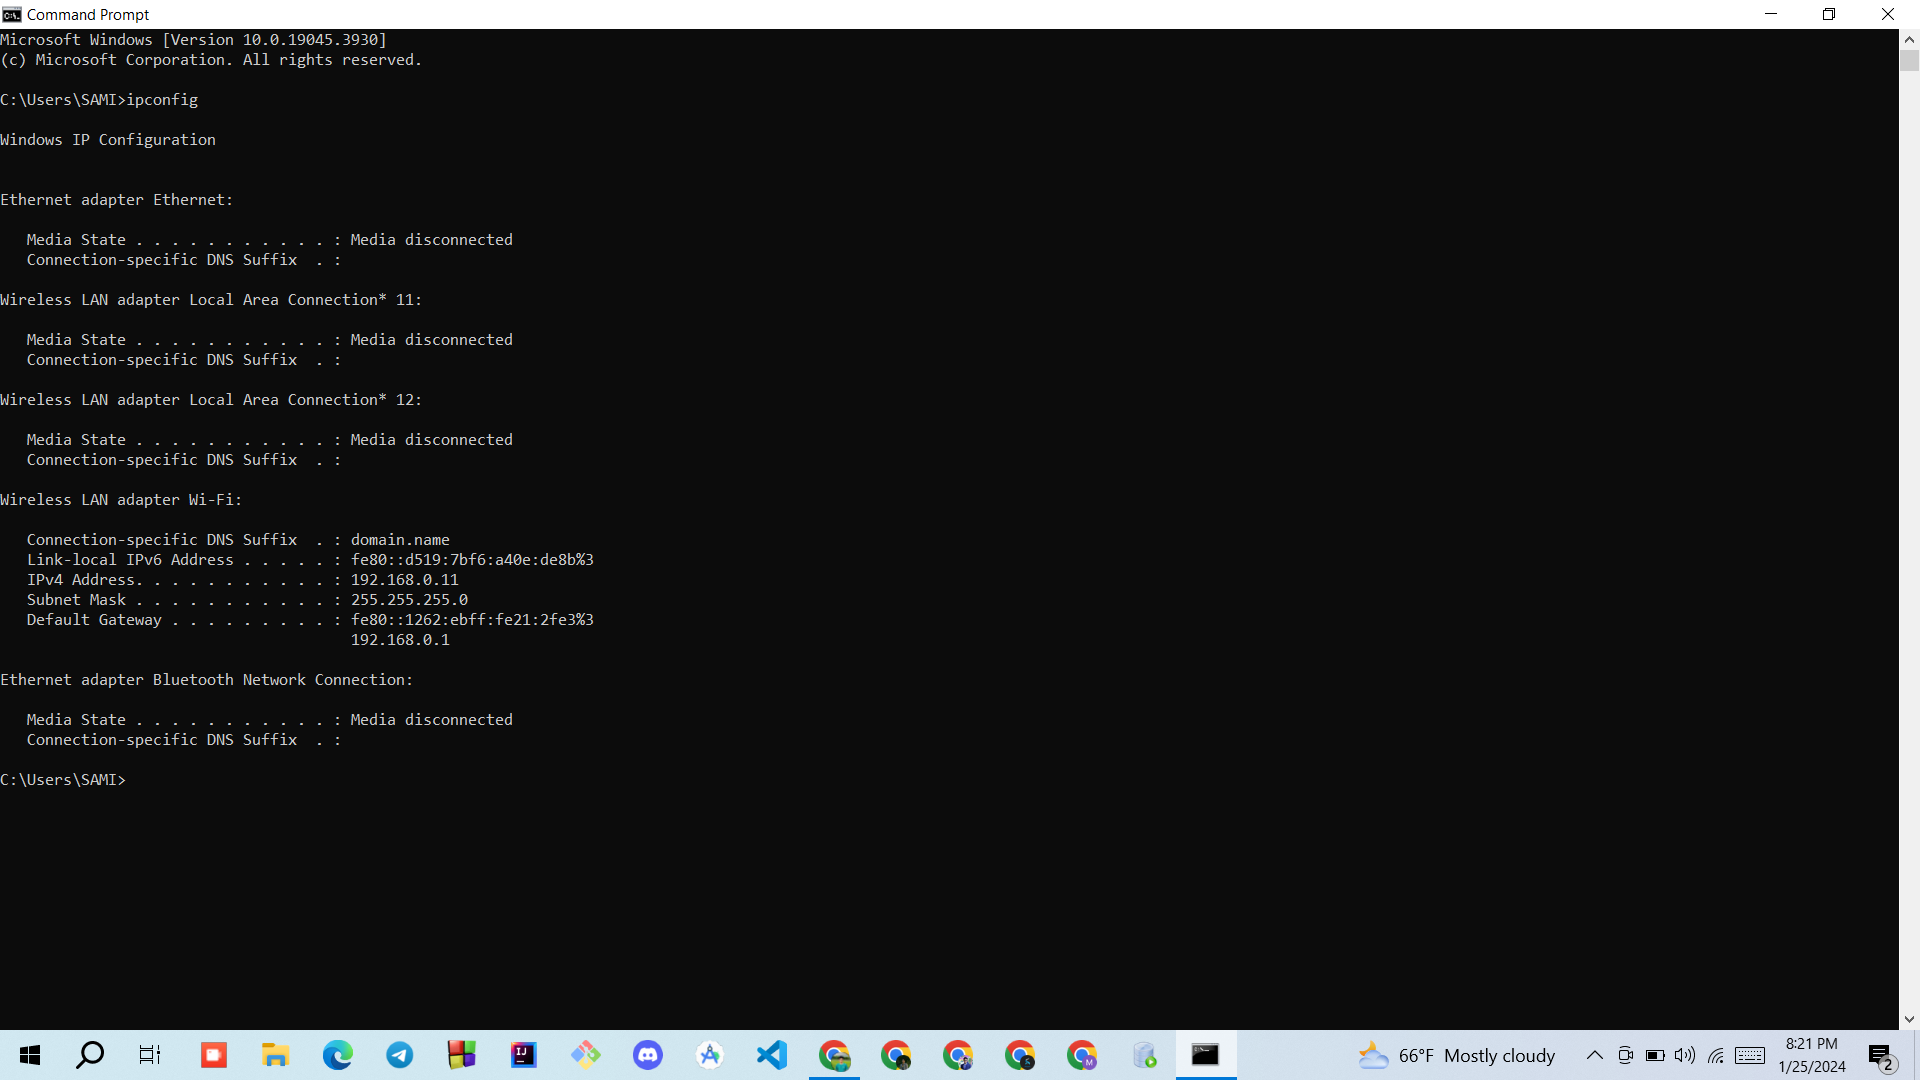
\includegraphics[width=\textwidth]{Screenshot (2).png}
\caption{Ifconfig Command}
\end{figure}

\begin{itemize}
  \item The `ipconfig` command in Windows provides essential information about a computer's network configuration.
  \item This includes its IP address, subnet mask, default gateway, and DNS servers.
  \item It is a valuable tool for diagnosing and troubleshooting network issues.
\end{itemize}


\subsection{}
\begin{figure}[!h]
\centering
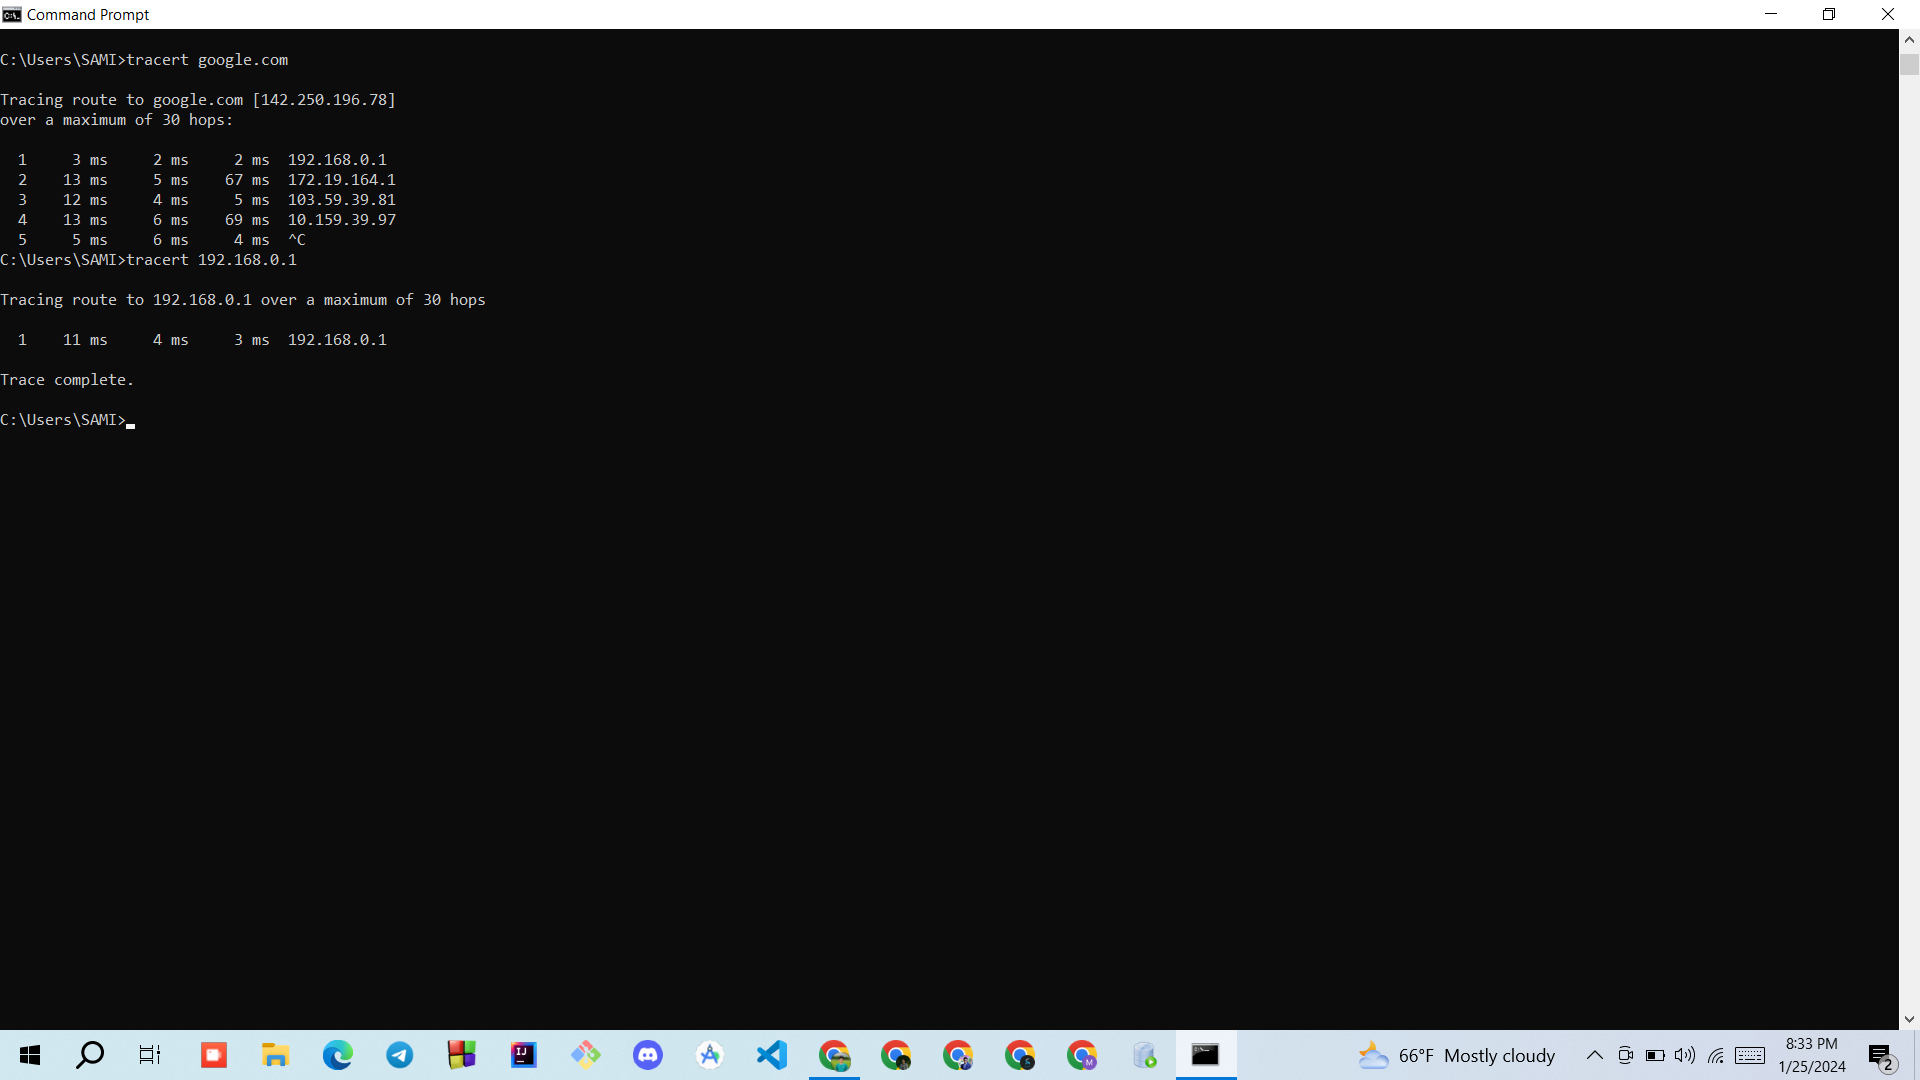
\includegraphics[width=\textwidth]{Screenshot (3).png}
\caption{Traceroute Command}
\end{figure}

\begin{itemize}
  \item The `tracert` command is a network utility used to trace the route that packets take to reach a destination.
  \item It shows the IP addresses of each hop along the way and the time it takes for packets to travel from the source to each intermediate destination.
  \item This tool is helpful for identifying network bottlenecks, locating connectivity issues, and understanding the path data takes through the network.
\end{itemize}



\subsection{}
\begin{figure}[!h]
\centering
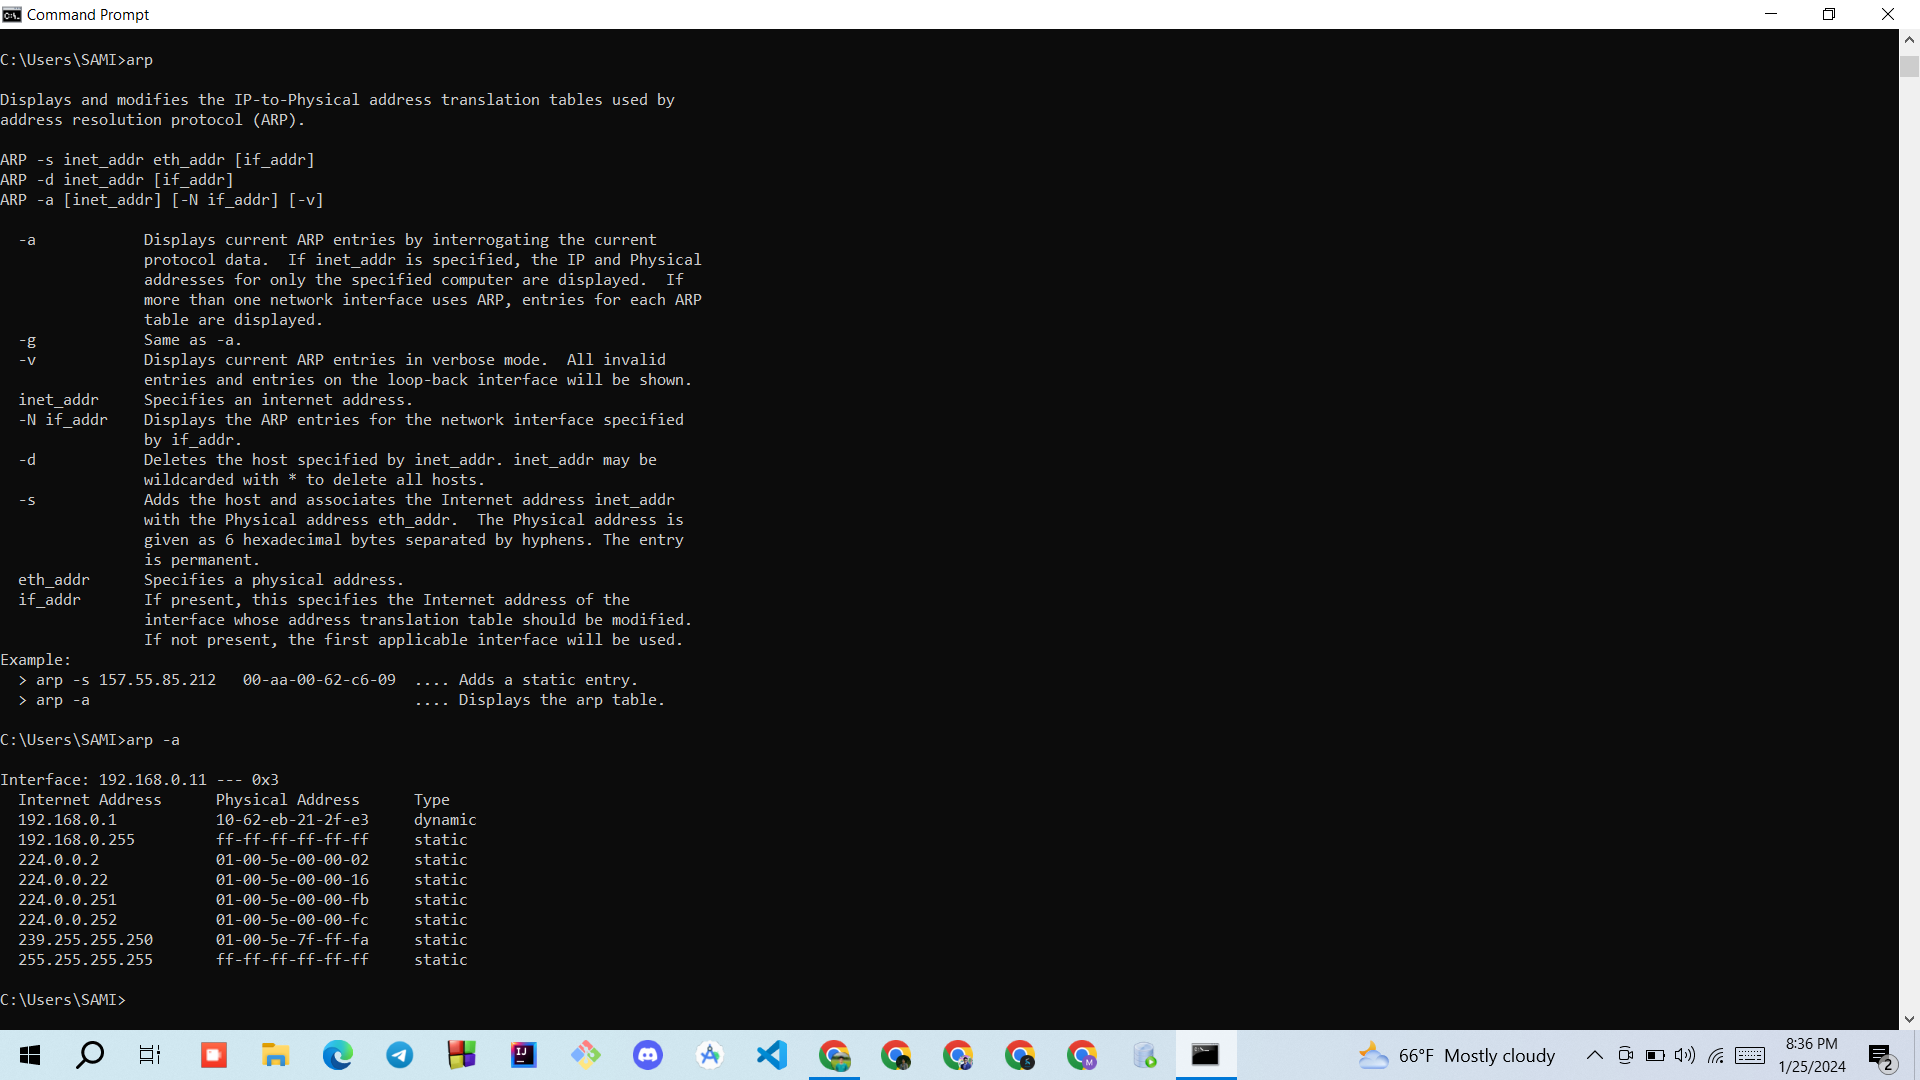
\includegraphics[width=\textwidth]{Screenshot (4).png}
\caption{ARP Command}
\end{figure}

\begin{itemize}
  \item The `arp` command is a network utility used to display and manage the Address Resolution Protocol (ARP) cache on a system.
  \item It shows the mapping between IP addresses and corresponding physical MAC addresses.
  \item This tool is essential for troubleshooting network connectivity issues, as it helps in identifying the devices present on the local network and their associated MAC addresses.
\end{itemize}



\subsection{}
\begin{figure}[!h]
\centering
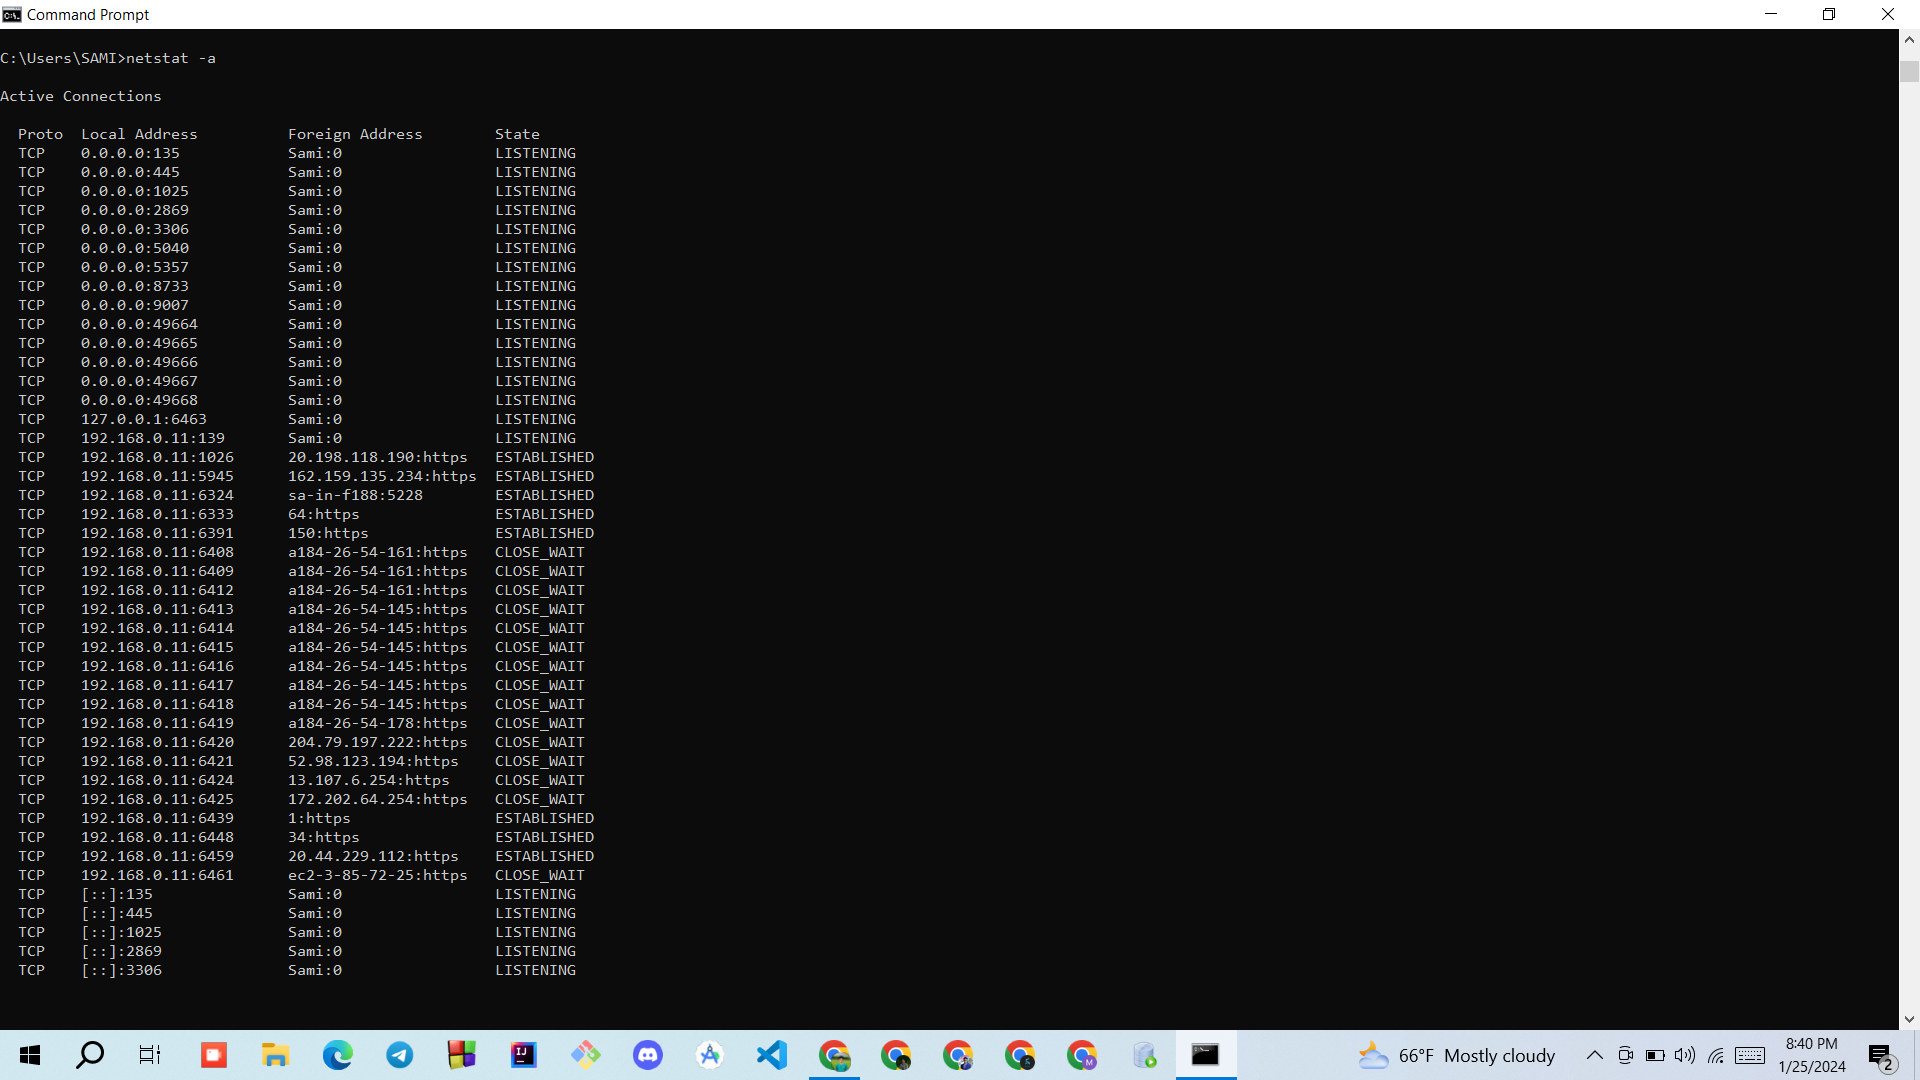
\includegraphics[width=\textwidth]{Screenshot (5).png}
\caption{Netstat Command}
\end{figure}

\begin{itemize}
  \item The `netstat` command is a network utility used to display active network connections, listening ports, and related information on a system.
  \item It provides details about established connections, listening ports, routing tables, and network interface statistics.
  \item This tool is valuable for diagnosing network issues, identifying open ports, and monitoring network activity on a computer.
\end{itemize}


\subsection{}
\begin{figure}[!h]
\centering
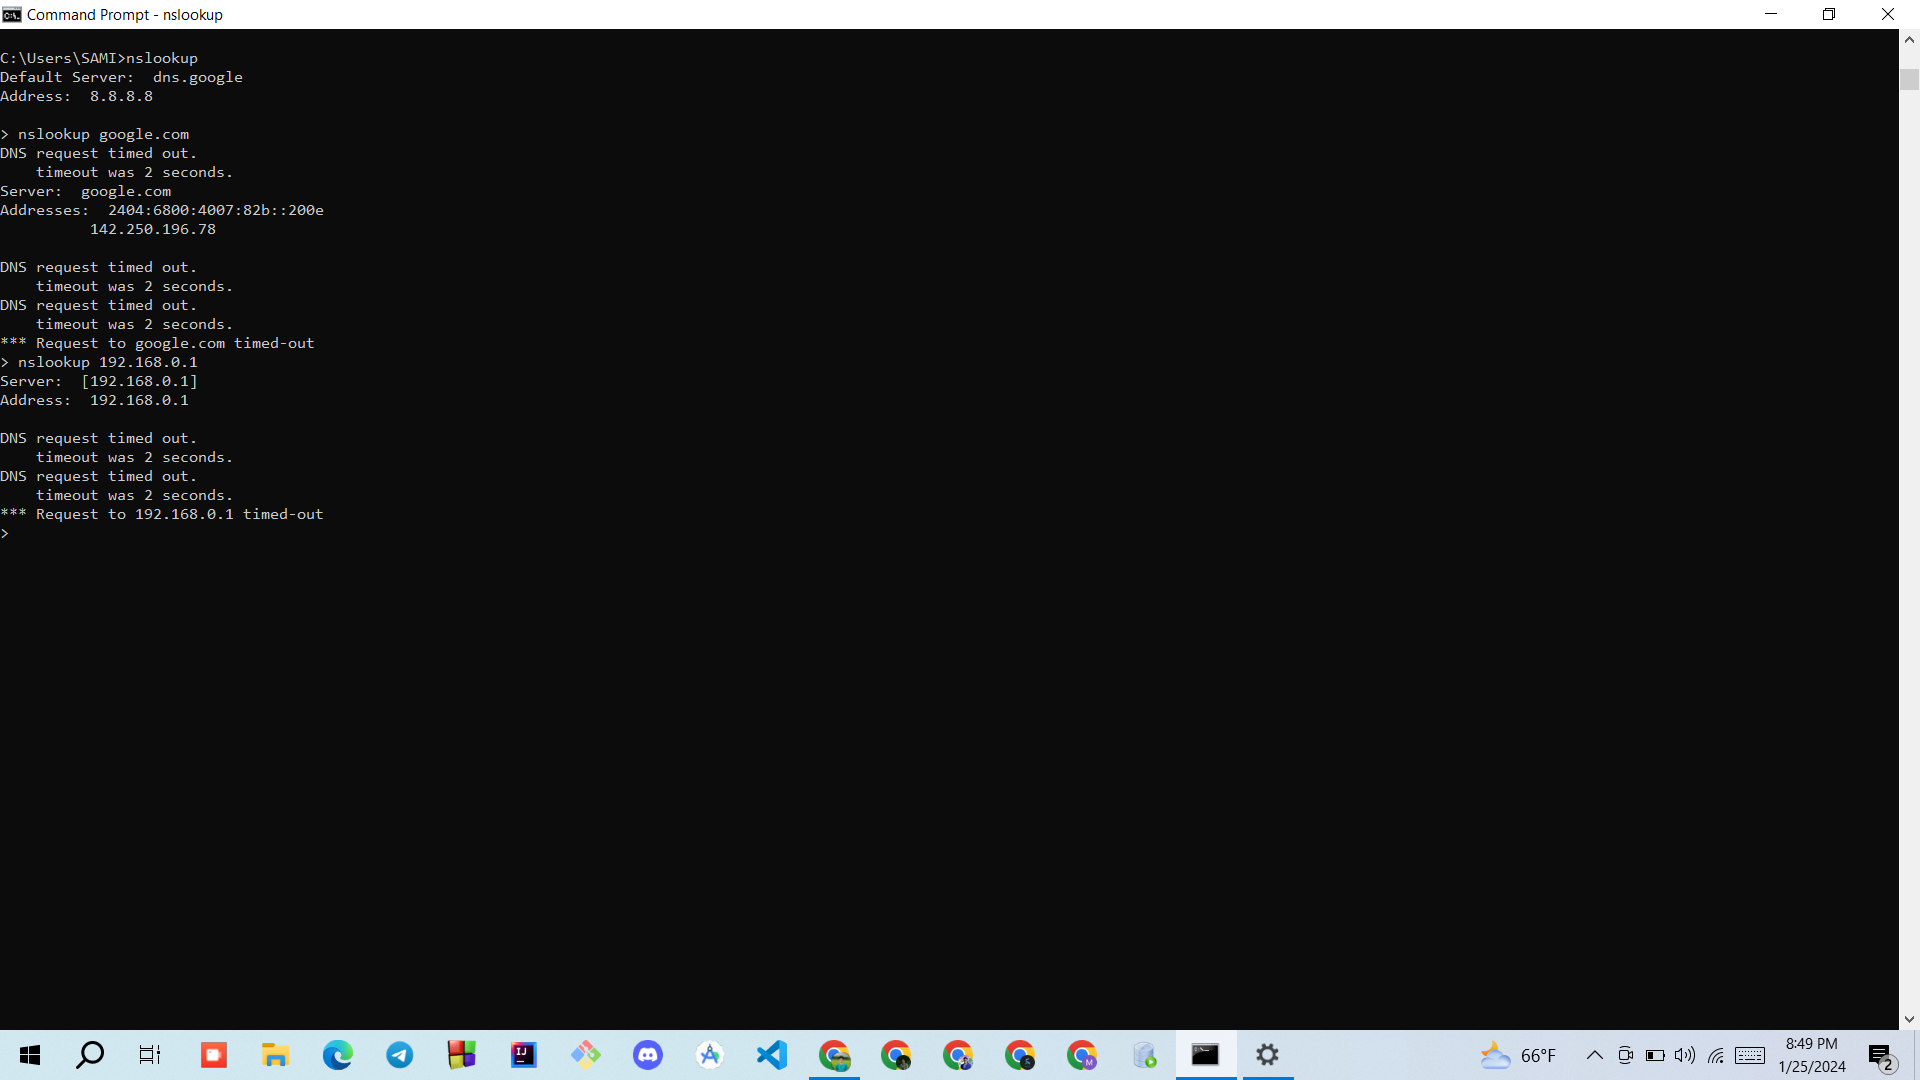
\includegraphics[width=\textwidth]{Screenshot (6).png}
\caption{Nslookup Command}
\end{figure}

\begin{itemize}
  \item The `nslookup` command is a network utility used for querying Domain Name System (DNS) servers to obtain information about domain names and IP addresses.
  \item It allows users to perform DNS lookups, find the IP address of a domain, and retrieve information about the DNS records associated with a specific hostname.
  \item This tool is useful for troubleshooting DNS-related issues, verifying DNS records, and obtaining information about domain name resolution.
\end{itemize}







\newpage
\section{Experience}
\begin{itemize}
  \item Explored practical examples to showcase the command's functionality.
  \item Tested the command on Linux, highlighting its usage and nuances.
  \item Recognized variations in command syntax when transitioning to the Windows environment.
  \item Emphasized the need for adaptability across different operating systems.
\end{itemize}


\begin{thebibliography}{1}
  %\bibitem{book} Computer networking: a top-down approach 6th ed.
  \bibitem{Commands} Windows IP Commands: \url{https://www.networkstraining.com/windows-ip-commands/}
  %\bibitem{W3School} HTML Codes: \url{http://www.w3schools.com/}
\end{thebibliography}


\end{document}